\section{Theoretical framework}
\label{sect:theoryframework}
There are two types of data storage, row-based and column-based data formats. Row-based data stores are considered the traditional approach where we data is written one row at a time. This makes it very easy to insert new data or modify an existing record. However, with a row-based store, more data is read than is needed resulting in overhead. Column-based data, on the other hand, writes the data vertically by column. The column-based approach ensures that you only need to read the data you are interested in. However, the downside of this method is that it requires multiple accesses in order to write the records since their columns are distributed in different sections. Figure \ref{fig:rowvscolumn} below is a visual representation of the description above (Graph replicated from the presentation "The future of column-oriented data processing with Arrow
and Parquet") \cite{jack_future_nodate, cao_data_2017}. 


\begin{figure}[!h]
  \centering
  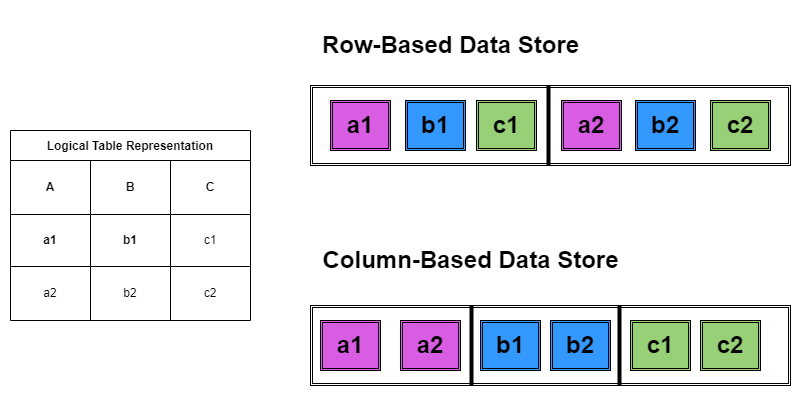
\includegraphics[width=0.7\textwidth]{img/concept.png}
  \caption{Row-based Data Store vs column-based data store. Replicate from \cite{jack_future_nodate}}
  \label{fig:rowvscolumn}
\end{figure}

\subsection{Column-based data formats}

The columnar data formats are a popular choice for fast analytic workloads. As opposed to row-oriented storage, columnar storage can significantly reduce the amount of data fetched from disk by allowing access to only the columns that are relevant to the particular query or workload. Moreover, columnar storage combined with efficient encoding and compression techniques can drastically reduce the storage requirements without sacrificing query performance \cite{floratou2018columnar}. It is worth noting that columnar data formats are suitable for large data volumes and read-only intensive workloads \cite{jack_future_nodate, cao_data_2017}. 

\subsubsection{Parquet}
Apache Parquet is a column-based serialization format mainly used in the Hadoop ecosystem, regardless of the choice of data processing framework, data model, or programming language \cite{vohra_apache_2016}. Parquet is built to support very efficient compression and encoding schemes. Instead of simply flattening the nested namespaces, it uses the record shredding and assembly algorithm described in the Dremel paper\cite{36632}. Multiple projects have demonstrated the performance impact of applying the right compression and encoding scheme to its data. Some projects, such as WikiParq, is an interesting project that builds on top of the Parquet format to tabulate and package the Wikipedia corpora\cite{klang_wikiparq_2016}. Its content can then be extracted by querying the database to obtain the exact information the user needs. Besides the points above, Parquet also allows for compression schemes to be specified on a per-column level, and is future-proofed to allow adding more encoding as they are invented and implemented \cite{vohra_apache_2016, cao_data_2017}.

\subsection{Row-based data formats}
Row-based data formats are ideal for visual data representation as well as transnational query. Examples of data formats used for visual data representation are csv and xlsx. Row-based formats are also very efficient and suitable for smaller data volumes. Below follows a presentation of each row-based data format that is to be benchmarked \cite{vohra_apache_2016_avro, cao_data_2017}.

\subsubsection{Avro}
Apache Avro is a compact binary data serialization format that provides various data structures and row-wise serialization\cite{vohra_apache_2016_avro}. Avro uses the JSON notation schema to serialize and deserialize data. Unlike some other similar systems, such as Google Protobuf, Avro does not require code generation and uses dynamic typing. Data are not tagged because the schema is accompanied with the data, resulting in a more compact data file. Avro supports versioning, so different versions of Avro data files can coexist along with their schemes. Since Avro is an Apache open-source project, many Apache projects support the Avro format such as Apache Hive, which provides support to store a table as Avro. Apache Flume supports Avro as input and output \cite{vohra_apache_2016, vohra_apache_2016_avro, cao_data_2017}. 

\subsubsection{CSV}
\gls{CSV} is a very simple format where each record is located on a separate line, delimited by a line break (CRLF) \cite{shafranovich_common_2005}. Although simple, the format has been used to exchange and convert data between various spreadsheet programs. It is also very widely used as the format for storing and distributing data in the open-source data science community \cite{shafranovich_common_2005, cao_data_2017}.

\subsubsection{Open Office XML-based spreadsheet format-XLSX}
The Open Office XML-based spreadsheet format that uses .xlsx as a file extension has been the default format produced for new documents by Microsoft Excel versions since Excel 2007 \cite{noauthor_xlsx_2022}. The format was designed to be equivalent to the binary .xls format produced by earlier versions of Microsoft Excel \cite{noauthor_xlsx_2022, cao_data_2017}. 

\subsection{Previous comparative studies}
Several previous studies have done research in this field. For example, Plase et al. compared Avro and Parquet with respect to text formats to evaluate the performance of the data queries \cite{plase_comparison_2017}. Different data query patterns have also been evaluated in this study. Blomer performed a quantitative review on some common data formats, including Parquet and Avro, with respect to \gls{HEP} datasets, which consist of n-tuples and \glspl{AOD}, and lots of numerical data\cite{blomer_quantitative_2018}. Todor Ivanov and Matteo Pergolesi have in a journal article reasoned about the impact of using columnar-based file formats with SQL for Hadoop Engine performance, mainly comparing the ORC format vs Parquet \cite{ivanov_impact_2020, cao_data_2017}.
